% Template for URSI Student Paper Competition
%
% Use pdflatex or latex + dvips + ps2pdf to produce a PDF.
%
% 

\documentclass[spc]{ursi}
\fancyfoot{} \fancyfoot[C]{\thepage} %remove copyright footer, add pagenumber
%% Add packages and define personal macros here, but ensure that they do not
%% interfere with the fonts and page layout. Do not add hyperlinks.

\title{Template for URSI Student Paper Competition}

%% Use \affref{nn} and matching \aff{nn}{...} below for several authors
%% Mark the presenting author with an asterisk
\author{First A. Author\affref{ref1}, Second B. Author*\affref{ref1},
  and Third C. Author\affref{ref2}}

%% define affiliations and addresses
\affiliation{%
  % use explicit line-breaks \\ if needed
  \aff{ref1}{ABC University, Prague, Czechia; e-mail: FAA@seznam.cz; SBA@email.cz}
  \aff{ref2}{The Next University, Neverland, USA; e-mail: TCA@gmail.com}
}

% (Omit \affref and \aff and the asterisk if there is only one author.)

\begin{document}

\maketitle

\begin{abstract}
  These instructions provide guidance and a template for
  the preparation of a paper for URSI Student Paper Competition.
\end{abstract}

\section{Introduction}

These instructions provide guidance for the preparation of your paper for URSI Student Paper Competition. The margins and required spacing between different
sections are demonstrated for author's convenience. To insert your text
just highlight each section and replace with your own text. Otherwise, use
this as a guideline to compare your final document in terms of margins,
font sizes, and spacings.

\section{Layout}

The URSI Student Paper Competition (SPC) paper should be single spaced,
single column and \textbf{sized for A4 paper} according to this
template. The paper should be no longer than \textbf{10 pages}.

The body text should be Times New Roman 10~pt. Sections should be titled
and numbered in bold Times New Roman 12~pt.  The top and bottom margins
should be 2.5~cm (1~inch); the left- and right-hand margins should be
1.6~cm (0.63~inch).  Paragraphs should be separated with one blank line. Do
not indent paragraphs.

The title should be centered according to this template. The author's (or
authors') name and complete organizational affiliation should be two lines
below the title. If there are multiple authors, the presenter is to be
identified with an asterisk.  The text should start three lines below the
last name.

\section{Paper Content}

The paper should include an abstract and the usual sub sections and should
be in English.

Citations and references should follow IEEE format (as used by the
\emph{Radio Science Bulletin}).  Citations can be of the
form~\cite{cannon,mannix} as is appropriate to the sentence, with the
reference format illustrated at the end of this template.

\section{Equations}

Equations should be centered with the equation numbers right justified in
the following format:
\begin{equation}
  \label{eq:T}
  T' = \frac{r_\text{e}^2\lambda^2GC_\text{s}L
    \sec\theta\sqrt{\pi}\ \Gamma\!\left(\frac\rho2\right)}
  {4\pi^2\,\Gamma\!\left(\frac{\rho+1}{2}\right)}.
\end{equation}


\section{Figures and Tables}

\subsection{Figures}

Figures should include a caption beneath the figure (in Times Roman 10 pt.)
and the caption should include the Figure number in
bold. Figure~\ref{fig:asc} provides an example.

\begin{figure}[tbp]
  \centering
  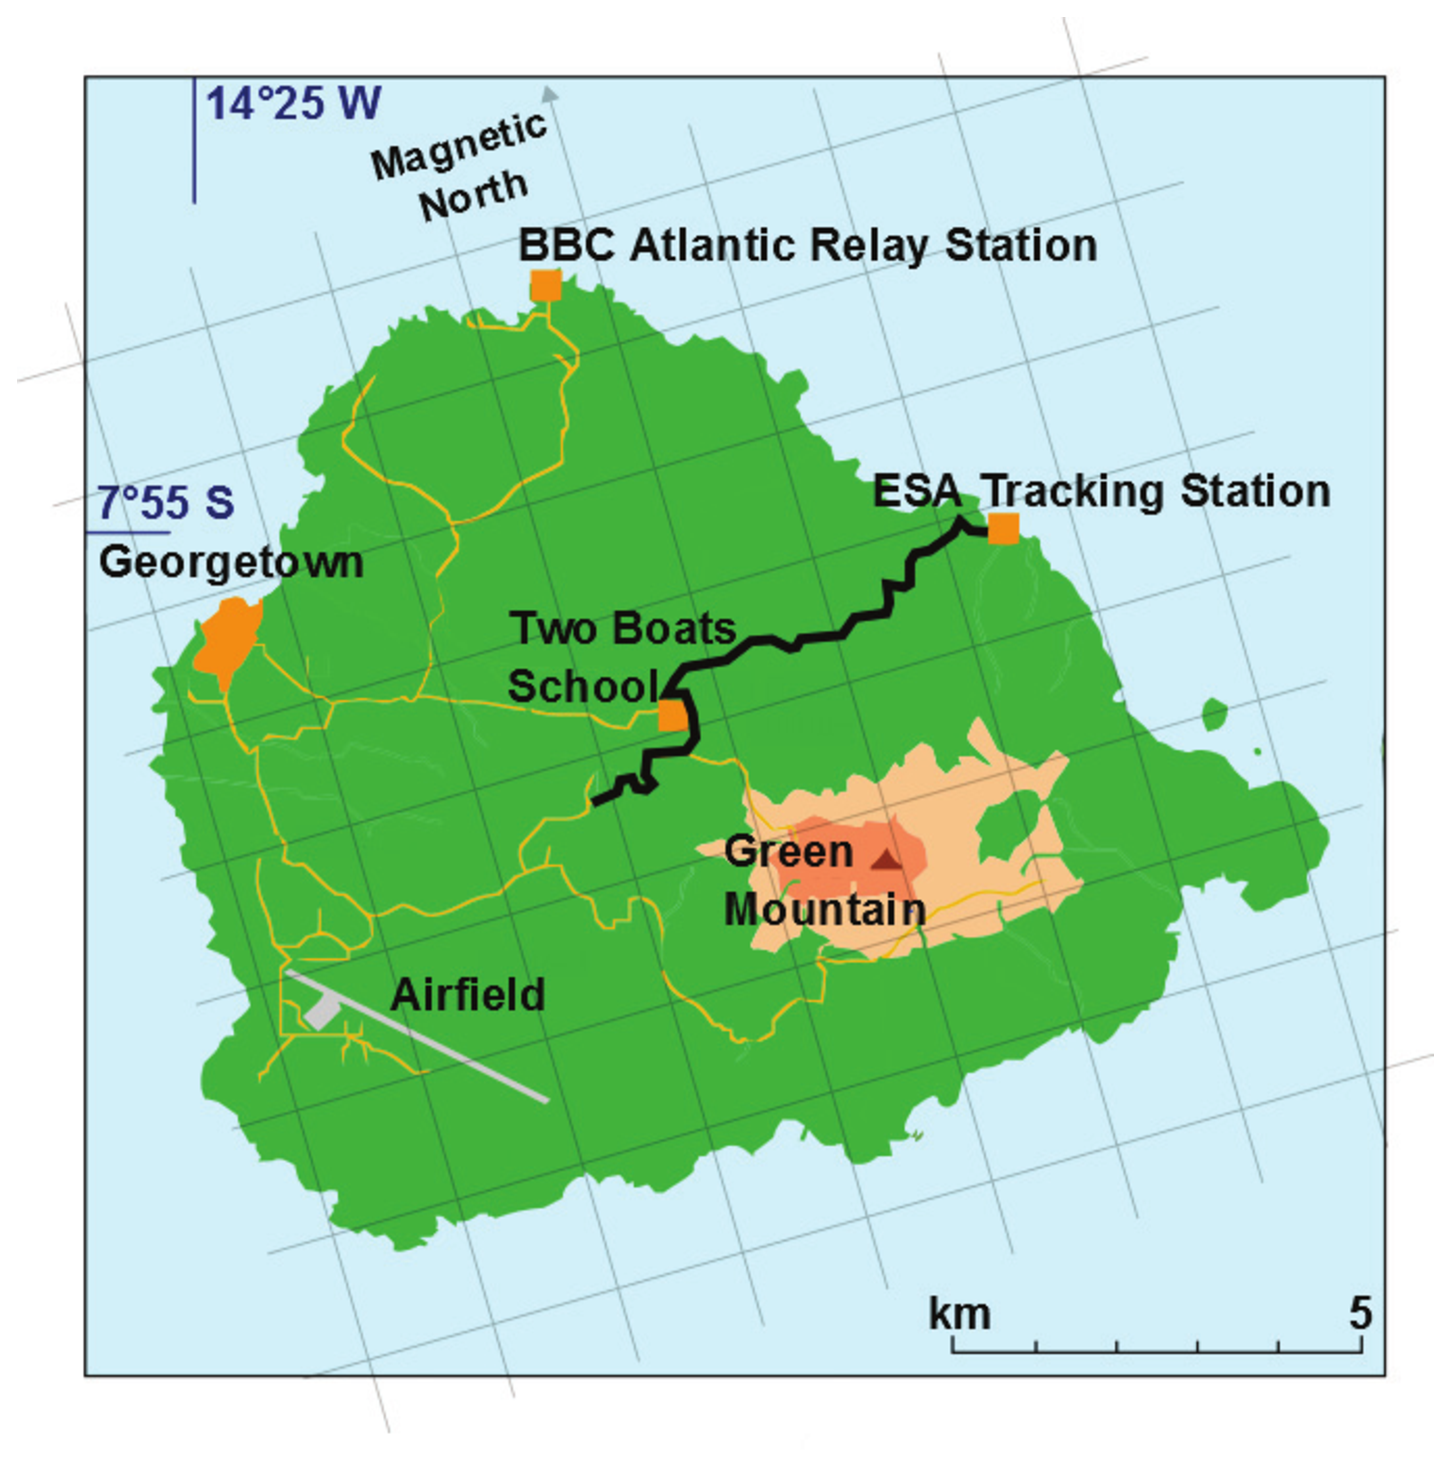
\includegraphics[width=77mm]{ascension_island}
  \caption{Ascension Island (7.9\textdegree S, 14.8\textdegree W showing
    the ESA Tracking Station which was the location of the fixed receiver
    and the road (shown in black) along which the mobile measurements were
    made).}
  \label{fig:asc}
\end{figure}

\subsection{Tables}

Likewise, tables should include a caption (in Times Roman 10 pt.) but this
time above the table. The caption should include the table number in bold.

\section{Export}
All submissions will be electronic and in a PDF format (*.pdf) and all
fonts must be embedded in the submitted PDF document.

Embedded Type 1 or True Type fonts are required in the submitted PDF file
as subset fonts. Type 3 fonts (bitmaps) will not be accepted. 

\section*{Acknowledgements}

Acknowledgements go in here.

\begin{thebibliography}{99}
\bibitem{cannon} P. S. Cannon, ``Extreme Space Weather --- A Report
  Published by the UK Royal Academy of Engineering,'' \emph{Space Weather},
  \textbf{11}, 4, April 2013, pp. 138--139, doi:10.1002/swe.20032.
\bibitem{mannix} C. R. Mannix, D. P. Belcher, P. S. Cannon, and
  M. J. Angling, ``Using GNSS Signals as a Proxy for SAR Signals:
  Correcting Ionospheric Defocusing,'' \emph{Radio Science}, \textbf{51},
  2, February 2016, pp. 60--70, doi: 10.1002/2015RS005822.
\end{thebibliography}




\end{document}
